%
% common information to the web version and book version
%
% images will be imported by searching the paths set with \graphicspath
% the book.tex or web.tex sets this so the correct resolution images end
% up in the correct document.
% 
% cover is done elsewhere, as this is usually broken out from the 
% ``text block'' for POD publishing--see book.tex
%
\newcommand{\signed}[1]{\par\hfill\normalfont--- \textit{#1}}

\newpage

\vspace*{1in}
\begin{center}
{\Large from the Carpentries} 

{\LARGE for Greg}

{\large (who would have `enjoyed' typesetting this book)}

\vspace*{0.5in}

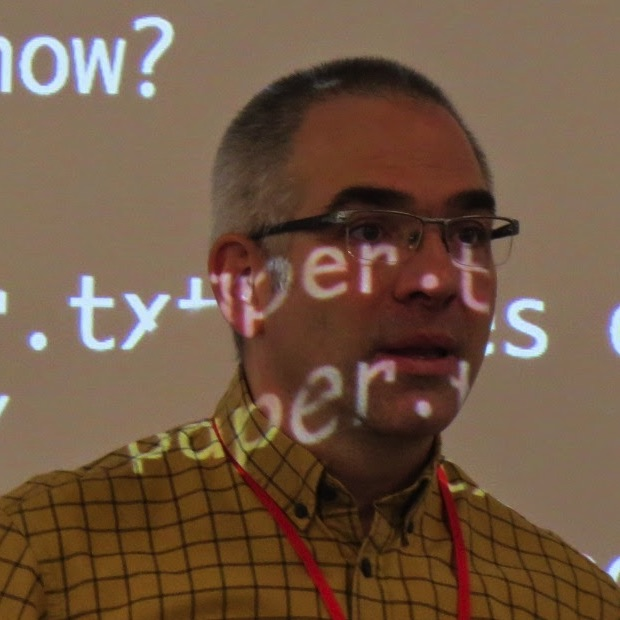
\includegraphics[width=3in]{gvwilson-tgac-large}
\end{center}
\newpage

\vspace*{1in}
{\LARGE About this book}

% TODO: Some brief introductory text here

\newpage

\pagestyle{plain}
% Russell Alleen-Willems
\begin{minipage}{0.45\textwidth}
    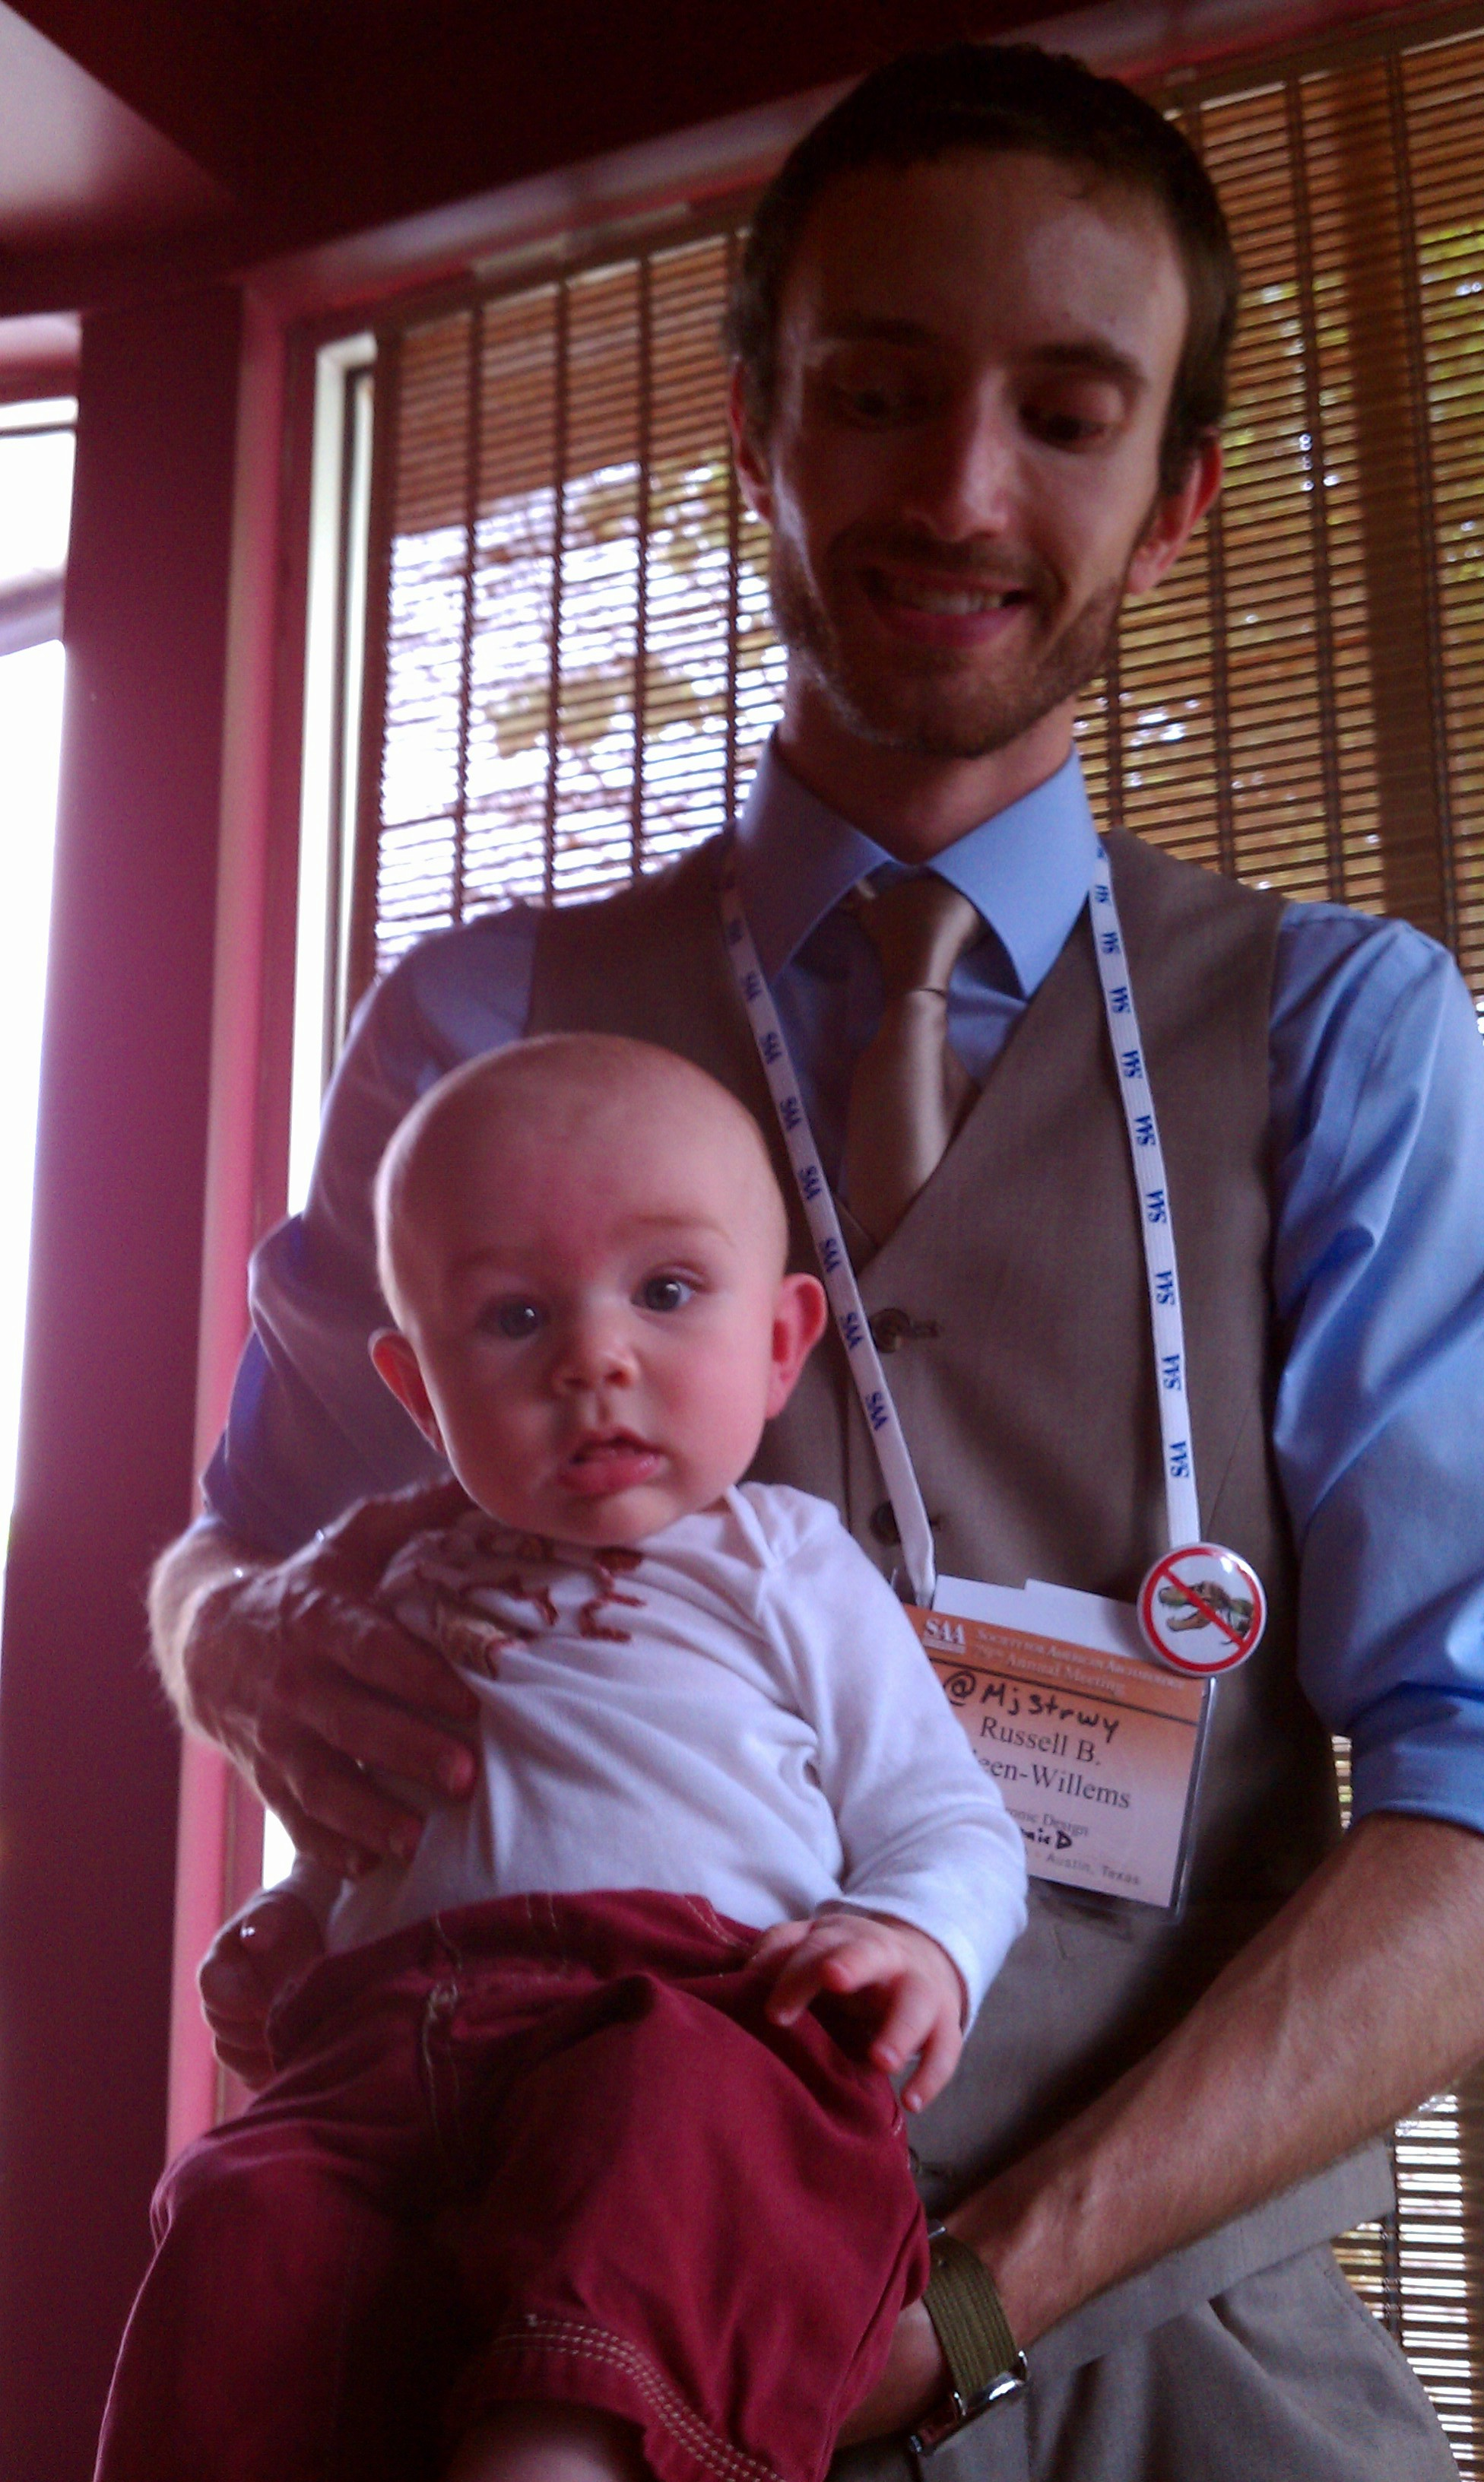
\includegraphics[width=3in]{russell}
\end{minipage}
\hfill
\begin{minipage}{0.45\textwidth}
\setlength{\parindent}{0in}
\setlength{\parskip}{1em}
I first met Greg during the 2014 Software Carpentry Instructor Training he held
online. I was a stay at home dad at the time and split my time between work
projects and watching my newborn son, Nova. Often I would have to attend
the SWC training sessions with my son napping in his baby carrier strapped
to my chest. Nova slept pretty well, and I tried to make judicious use of
the mute button so the session wasn't filled with baby noises. 

Greg, as a father himself, not only tolerated my son being in class with
me, but even seemed happy that he was there. Sometimes Greg also had to
teach with his daughter in tow if she was home ill. It was good for me to
see Greg model how being a scientist and active leader can mesh with the
other important roles in our lives. 

Thanks for all your hard work Greg, and best of luck in your future endeavors! 

[Photo is of me at the Society for American Archaeology conference with my son
in tow. I couldn't find a good picture of me and Nova at a SWC session, either
remote or in-person]

\signed{Russell Allen-Willems}
\end{minipage}

\newpage
% Carole Goble
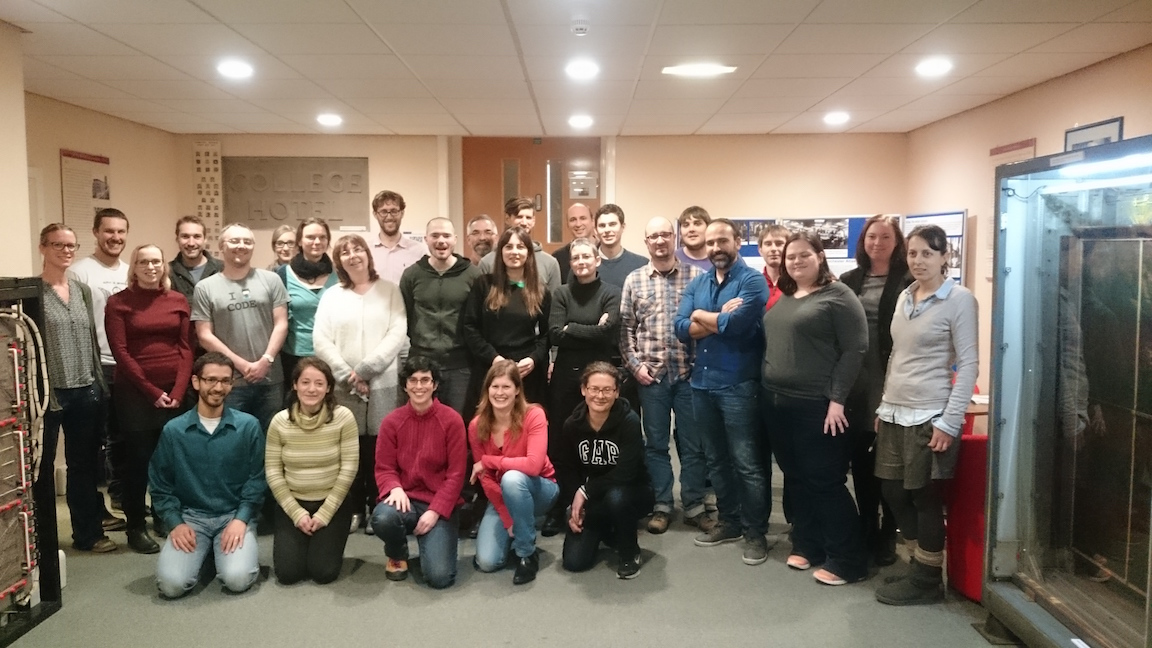
\includegraphics[width=8in]{carole-Instructor-Training-Manchester-2015-11-23}

I met Greg at  a conference in Chicago back in 2012. He was already a legend
and I was apprehensive - what could I do to help him with his mission? As part
of the Software Sustainability Institute, we were already working with Software
Carpentry. He was so inspirational, with such clarity of vision and passion. He
preached. I was blown away.  Meeting with Greg was like meeting with a force of
nature. From then on I was kind of working for him - helping set up SC across
the EU Life Science community through the ELIXIR programme and brokering
sponsorship deals and just doing my best  to promote SC. At a train the
trainers workshop in Manchester late 2015, I had the pleasure of seeing him in
action - handing on the wisdom. He challenged lazy thinking and easy practices,
and showed alternatives. Greg, you are one of the people who I can genuinely
say changed me. May you continue onwards and upwards.

\signed{Carole Goble}

\newpage
% Ian Hawke
\begin{figure}[h!]
\centering
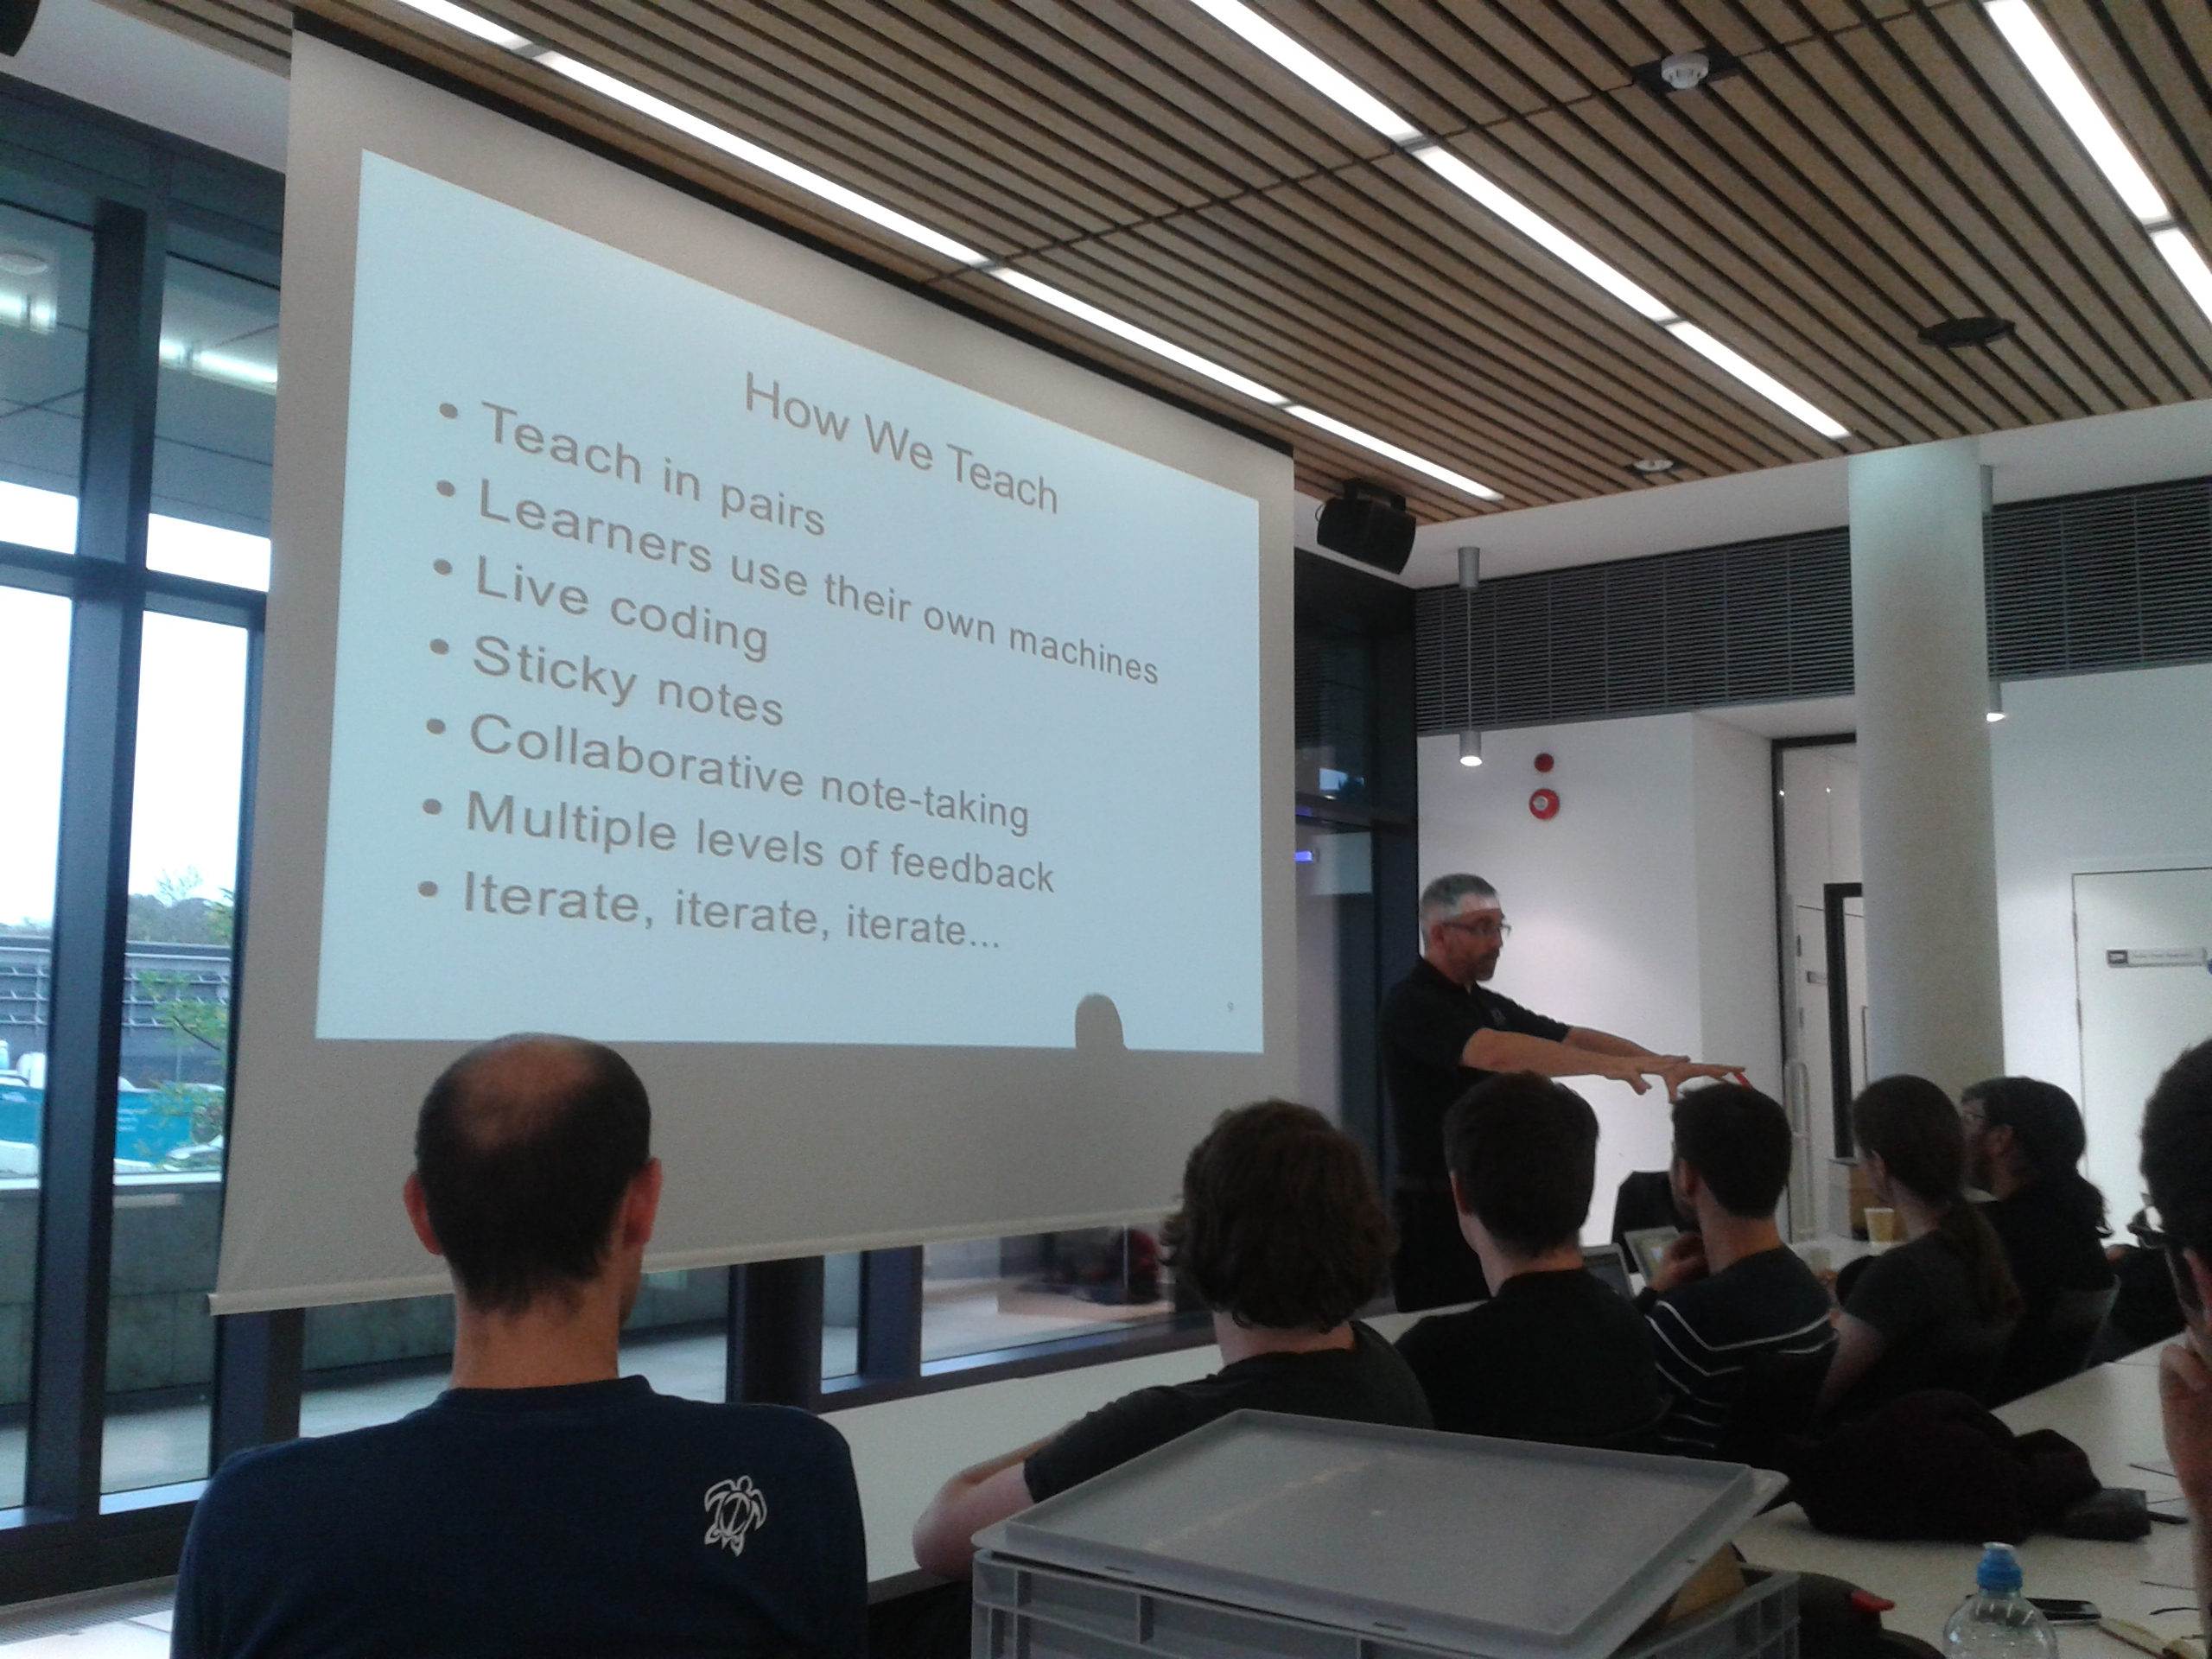
\includegraphics[width=8in]{ian-2015-11-10-Greg-Wilson.jpg}
\caption*{\textit{Greg mind-melds with a future instructor}}
\end{figure}
\vspace{-0.25cm}

In one amazing visit by Greg he gave me and our group of students loads of
ideas and enthusiasm, and then found time to talk me through a problem I had
with an ex-advisee. Above all he's given me the confidence to try something,
fail well, and then get back up and try again.

\signed{Ian Hawke}

\newpage
\vspace*{1in}

{\LARGE Technical Details}

The basic template for this book was put together by Eric Jeschke in
2009, as part of a ``Solo Photo Book Month'' project.  The original book
is titled \title{Chickens, Anyone?} and is a lovely recounting of his
family's adventures with raising chickens in their back yard.  The template
was pointed out to me (Erik) by Jonah Duckles, and by complete coincidence
I am personally acquainted with Eric Jeschke, and knowing of his talent I
immediately decided to adopt his work as my template, as he has made it
freely available for copying:

https://redskiesatnight.com/books/pod/latex-templates-for-pod-publishing-with-blurb-com

You'll note that much of the layout of the book was inspired by his book,
so credit where credit is due.

I did what I could with photos taken off the web, and some sent to me by
individual respondents.  Many of them will not be,
perfectionalistically-speaking, `print-quality', but they'll have to do given
that this was done on short time.

The book is written using \LaTeX with {\em xetex} and {\em xdvipdfmx} for
easier adjustments for dead tree publishing.  The font used is EB Garamond.
The book was made on Cygwin, and files were tracked in (I'm sorry to say) a
{\em git} repository.

%END
